\chapter{Funcionamiento de la Aplicación}

Para la aplicación de las pruebas se realizaron siete casos de prueba con diez iteraciones
cada una, para ver la eficiencia del buscador desarrollado y el actual
buscador de la biblioteca de la Universidad de Nariño\footnote{\url{http://biblioteca.udenar.edu.co:8085/bibliotecavirtual/}}.

Las pruebas se hicieron llevando los siguientes casos de prueba y se calificó
como éxito (E) o fracaso (F), teniendo en cuenta que el éxito se lo califica si
la búsqueda a realizar está en los quince primeros resultados.

\subsection{Casos de prueba}

\begin{description}
 \item [Búsqueda por título completo:] esta búsqueda se la realizó enviando la consulta con 
 el título exacto que aparece en la base de datos(tildes, signos de puntuación y comillas), dando como
 resultado que los dos sistemas se comportan de la misma manera como lo muestra la Tabla~\ref{tabla:p1} y Figura~\ref{figura:p1}.
 
 \begin{center}
\begin{table}[!ht]
\caption{Búsqueda por título completo} \label{tabla:p1}
\scalebox{0.7}{
\begin{tabular}{|p{1cm} | p{14cm} | p{1.5cm} | p{2cm} |}
\toprule
\textbf{No} & \textbf{Consulta} & \textbf{SAWA} & \textbf{Biblioteca} \\
\hline
 1 & MATE-KDD: UNA HERRAMIENTA GENERICA PARA EL DESCUBRIMIENTO DE REGLAS DE CLASIFICACION MEDIANAMENTE ACOPLADA AL SGBD POSTGRESQL & E & E \\
 \hline
 2 & TARIYKDD : UNA HERRAMIENTA GENERICA DE DESCUBRIMIENTO DE CONOCIMIENTO EN BASES DE DATOS DEBILMENTE ACOPLADA CON EL SGBD POSTGRESQL & E & E \\
 \hline
 3 & IMPLANTACION DE PRIMITIVAS SQL PARA EL DESCUBRIMIENTO DE REGLAS DE ASOCIACION Y CLASIFICACION & E & E \\
 \hline
 4 & ATLAS HERRAMIENTA DE CARTOGRAFIA WEB Y GEOCODIFICACION PARA EL DESARROLLO DE SISTEMAS HIBRIDOS EN AREAS URBANAS SOBRE J2EE Y POSTGRESQL & E & E\\
 \hline
 5 & GEOPASTO UN SISTEMA DE INFORMACION GEOGRAFICA WEB ORIENTADO AL APOYO PARA LA TOMA DE DECISIONES BASADOS EN EL PLAN DE ORDENAMIENTO TERRITORIAL & E & E \\
 \hline
 6 & SISTEMA DE INFORMACION PARA EL REGISTRO Y CONSULTA DEL MATERIAL DE BIBLIOTECA EN EL ENTORNO INTRANET DEL CENTRO SUR COLOMBIANO DE LOGISTICA INTERNACIONAL & E & E\\
 \hline
 7 & SISTEMA DE INFORMACION PARA LA BIBLIOTECA Y DESARROLLO DE LA PAGINA WEB DE LA UNIVERSIDAD DE NARIÑO -SEDE IPIALES & E & E\\
 \hline
 8 & ANALISIS, DISEÑO Y DESARROLLO DE UN SISTEMA DE INFORMACION MEDIANTE UNA RED DE COMUNICACIONES E INTERNET PARA LA ALCALDIA DE LINARES. & E & E\\
 \hline
 9 & SISTEMA DE INFORMACION PARA EL MANEJO CONTABLE DE LOS ALMACENES DEL GRUPO CABAL IPIALES & E& E\\
 \hline
 10 & DESARROLLO DE UN SISTEMA DE INFORMACION COMPUTARIZADO DE REGISTRO Y CONTROL ACADEMICO PARA EL POLITECNICO SAN JUAN DE PASTO & E& E\\
 \hline
\midrule
\bottomrule
\end{tabular}
}
\end{table}
\end{center}
 
 \begin{figure}[!ht]
\begin{center}
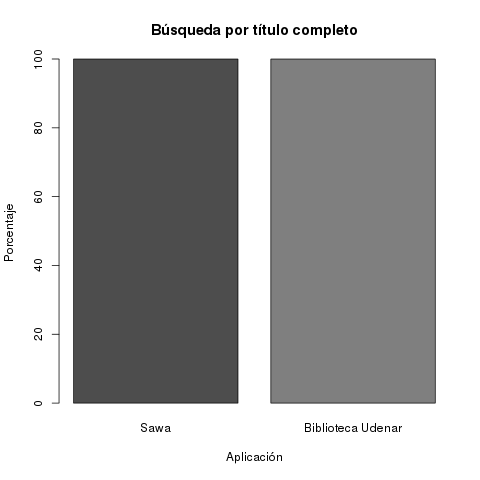
\includegraphics[width=8cm]{pictures/p1.png}
\end{center}
\caption{Búsqueda por título completo} \label{figura:p1}
\end{figure}

\newpage
  
 \item [Búsqueda por autor completo:] esta búsqueda se la realizó enviando la consulta con
 el autor exacto que aparece en la base de datos, dando como resultado que el sistema realizado
 en esta investigación de un resultado del 100\% y el sistema de biblioteca 40\% como lo muestra la Tabla~\ref{tabla:p2} y Figura~\ref{figura:p2}.
 
  \begin{center}
\begin{table}[!ht]
\caption{Búsqueda por autor completo} \label{tabla:p2}
\scalebox{0.7}{
\begin{tabular}{|c|l |c| c|}
\toprule
\textbf{No} & \textbf{Consulta} & \textbf{SAWA} & \textbf{Biblioteca} \\
\hline
 1 & CLAUDIA MILENA CASTRO RODRIGUEZ & E & F \\
 \hline
 2 & ANDRES OSWALDO CALDERON ROMERO & E & E \\
 \hline
 3 & STIVENSON ARMERO KREISBERGER & E & E \\
 \hline
 4 & CARLOS ERNESTO ARTEAGA NOGUERA & E & F \\
 \hline
 5 & JUAN CARLOS ROMAN FIGUEROA & E & E\\
 \hline
 6 & HECTOR EDMUNDO ROSERO CASTRO & E & F \\
 \hline
 7 & PAOLA MARY CORAL BASTIDAS & E & F\\
 \hline
 8 & OCTAVIO DELGADO ORDOÑEZ & E & E\\
 \hline
 9 & MARIA ELENA ESTRADA ESPAÑA & E & F\\
 \hline
 10 & YEIMY ANDRES ARTEAGA GUERRON& E& F\\
 \hline
\midrule
\bottomrule
\end{tabular}
}
\end{table}
\end{center}
 
 \begin{figure}[!ht]
\begin{center}
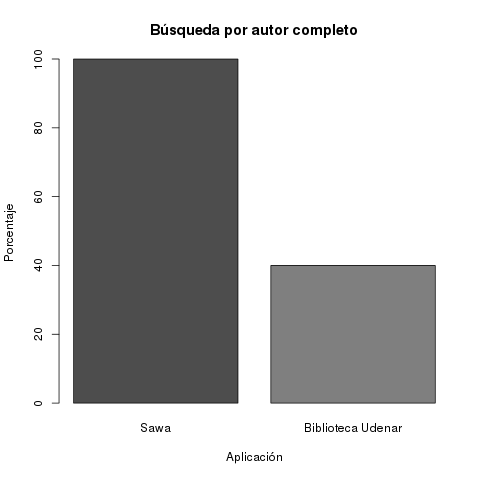
\includegraphics[width=8cm]{pictures/p2.png}
\end{center}
\caption{Búsqueda por autor completo} \label{figura:p2}
\end{figure}
 
 \newpage
 \item [Búsqueda por un nombre y un apellido:] esta búsqueda se la realizó enviando la consulta
 con un nombre y un autor unicamente, dando como resultado que el sitema realizado
 en esta investigación de un resultado del 90\% y el sistema de biblioteca 40\% como lo muestra la Tabla~\ref{tabla:p3} y Figura~\ref{figura:p3}.
 
  \begin{center}
\begin{table}[!ht]
\caption{Búsqueda por un nombre y un apellido} \label{tabla:p3}
\scalebox{0.7}{
\begin{tabular}{|c|l |c| c|}
\toprule
\textbf{No} & \textbf{Consulta} & \textbf{SAWA} & \textbf{Biblioteca} \\
\hline
 1 & CLAUDIA  RODRIGUEZ & E & F \\
 \hline
 2 & ANDRES CALDERON & E & E \\
 \hline
 3 & STIVENSON KREISBERGER & E & E \\
 \hline
 4 & CARLOS   NOGUERA & E & F \\
 \hline
 5 & JUAN FIGUEROA & E & E\\
 \hline
 6 & HECTOR  ROSERO & E & F \\
 \hline
 7 & MARY CORAL & E & F\\
 \hline
 8 & OCTAVIO DELGADO & E & E\\
 \hline
 9 & ELENA  ESPAÑA & F & F\\
 \hline
 10 & YEIMY  ARTEAGA & E& F\\
 \hline
\midrule
\bottomrule
\end{tabular}
}
\end{table}
\end{center}
 
 \begin{figure}[!ht]
\begin{center}
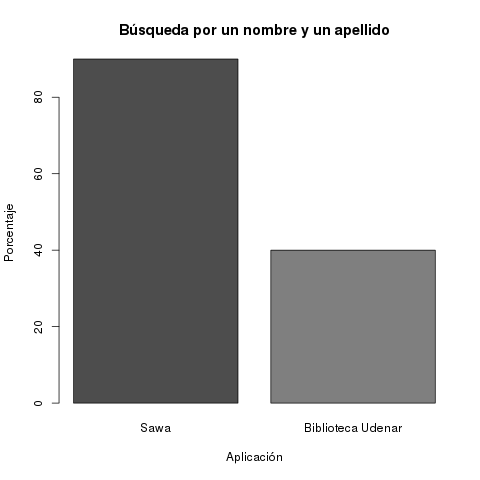
\includegraphics[width=8cm]{pictures/p3.png}
\end{center}
\caption{Búsqueda por un nombre y un apellido} \label{figura:p3}
\end{figure}
 
 \newpage
 \item [Búsqueda por palabras contenidas en el título:] esta búsqueda se la realizó enviando la consulta
 con palabras que estén contenidas en el título, las palabras podían haberse enviado en el ordén del
 título como en desorden, dando como resultado que el sitema realizado
 en esta investigación de un resultado del 100\% y el sistema de biblioteca 0\% como lo muestra la Tabla~\ref{tabla:p4} y Figura~\ref{figura:p4}.
 
    \begin{center}
\begin{table}[!ht]
\caption{Búsqueda por palabras contenidas en el título}  \label{tabla:p4}
\scalebox{0.7}{
\begin{tabular}{|c|l |c| c|}
\toprule
\textbf{No} & \textbf{Consulta} & \textbf{SAWA} & \textbf{Biblioteca} \\
\hline
 1 & REGLAS GENERICAS DE CLASIFICACION & E & F \\
 \hline
 2 & CONOCIMIENTO ACOPLADO A UNA BASE DE DATOS & E & F \\
 \hline
 3 & PRIMITIVAS PARA EL DESCUBRIMIENTO DE REGLAS & E & F \\
 \hline
 4 & CARTOGRAFIA Y GEOCODIFICACION WEB & E & F\\
 \hline
 5 & GEOPASTO ORIENTADO ALA TOMA DE DECISIONES & E & F \\
 \hline
 6 & REGISTRO  DEL MATERIAL DE BIBLIOTECA & E & F\\
 \hline
 7 & DESARROLLO DEL SISTEMA  PARA LA BIBLIOTECA & E & F\\
 \hline
 8 & ANALISIS Y DESARROLLO DE UNA UNA RED DE COMUNICACIONES & E & F\\
 \hline
 9 & SISTEMA PARA EL MANEJO CONTABLE DEL GRUPO CABAL & E& F\\
 \hline
 10 & SISTEMA DE INFORMACION DE REGISTRO Y CONTROL ACADEMICO & E& F\\
 \hline
\midrule
\bottomrule
\end{tabular}
}
\end{table}
\end{center}
 
  \begin{figure}[!ht]
\begin{center}
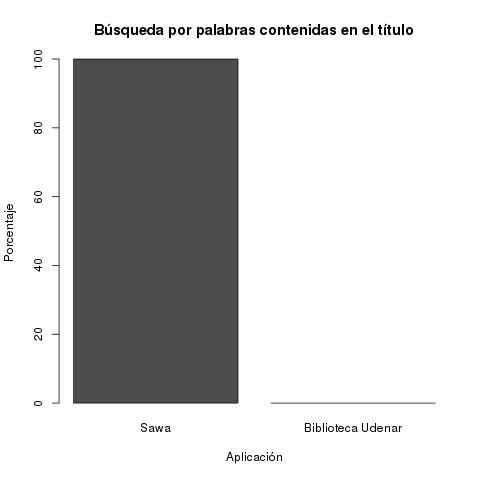
\includegraphics[width=8cm]{pictures/p4.png}
\end{center}
\caption{Búsqueda por palabras contenidas en el título} \label{figura:p4}
\end{figure}
 
 \newpage
 \item [Búsqueda por error ortográfico en el título:] esta búsqueda se la realizó enviando la consulta
 con uno o dos errores de digitación en el título, dando como resultado que el sitema realizado
 en esta investigación de un resultado del 100\% y el sistema de biblioteca 0\% como lo muestra la Tabla~\ref{tabla:p5} y Figura~\ref{figura:p5}.
 
 \begin{center}
\begin{table}[!ht]
\caption{Búsqueda por error ortográfico en el título} \label{tabla:p5}
\scalebox{0.7}{
\begin{tabular}{|p{1cm} | p{14cm} | p{1.5cm} | p{2cm} |}
\toprule
\textbf{No} & \textbf{Consulta} & \textbf{SAWA} & \textbf{Biblioteca} \\
\hline
 1 & MATE-KDD UNA HERRAMIENTA GENERICA PARA EL DESCUBRIMIENTO DE REGLOS DE CLASIFICACION MEDIANAMENTE ACOPLADA AL SGBD POSTGRESQL & E & F \\
 \hline
 2 & TARIYKDD UNA HERRAMIENTA GENERICA DE DESCUBRIMIENTO DE CONOCIMENTO EN BASES DE DATOS DEBILMENTE ACOPLADA CON EL SGBD POSTGRESQL & E & F\\
 \hline
 3 & IMPLANTACION DE PRIMITIVAS SQL PARA EL DESCUBRIMINTO DE REGLAS DE ASOSIASION Y CLASIFICACION & E & F \\
 \hline
 4 & ATLAS HERRAMIENTA DE CARTOGAFIA WEB Y GEOCODIFICACION PARA EL DESARROLLO DE SISTEMAS HIBRIDOS EN AREAS URBANAS SOBRE JEE Y POSTGRES & E & F\\
 \hline
 5 & GEOPATO UN SISTEMA DE INFORMACION GEOGAFICA WEB ORIENTADO AL APOYO PARA LA TOMA DE DECISIONES BASADOS EN EL PLAN DE ORDENAMIENTO TERRITORIAL & E & F \\
 \hline
 6 & SISTEMA DE INFORMACIOM PARA EL REGISTRO Y CONSULT DEL MATERIAL DE BIBLIOTECA EN EL ENTORNO INTRANET DEL CENTRO SUR COLOMBIANO DE LOGISTICA INTERNACIONAL & E & F\\
 \hline
 7 & SISTEMA DE INFORMACION PARA LA BIBLIOTECA Y DESARROLLO DE LA PAGINA WEB DE LA UNIVERSIDAD DE NARINO IPIALES & E & F\\
 \hline
 8 & ANALISIS DISENO Y DESARROLLO DE UN SISTEMA DE INFORMACION MEDIANTE UNA RED DE COMUNICASIONES E INTERNET PARA LA ALCALDIA DE LINARES. & E & F\\
 \hline
 9 & SISTEMA DE INFORMACION PARA EL MANEJO CONTABE DE LOS ALMASENES DEL GRUPO CABAL IPIALES & E& F\\
 \hline
 10 & DESARROLLO DE UN SISTEMA DE INFORMACION COMPUTALIZADO DE REGISTRO Y CONTROL ACADEMIC PARA EL POLITENICO SAN JUAN DE PASTO & E& F\\
 \hline
\midrule
\bottomrule
\end{tabular}
}
\end{table}
\end{center}
 
  
  \begin{figure}[!ht]
\begin{center}
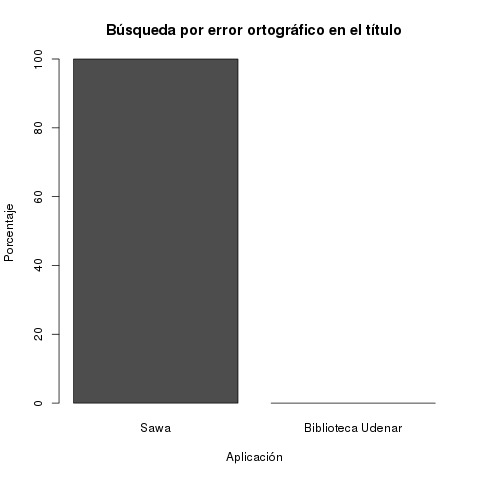
\includegraphics[width=8cm]{pictures/p5.png}
\end{center}
\caption{Búsqueda por error ortográfico en el título} \label{figura:p5}
\end{figure}

 \newpage
 \item [Búsqueda por error ortográfico en el autor:] esta búsqueda se la realizó enviando la consulta
 con uno o dos errores de digitación en el auto, dando como resultado que el sitema realizado
 en esta investigación de un resultado del 100\% y el sistema de biblioteca 0\% como lo muestra la Tabla~\ref{tabla:p6} y Figura~\ref{figura:p6}.
 
  \begin{center}
\begin{table}[!ht]
\caption{Búsqueda por error ortográfico en el autor} \label{tabla:p6}
\scalebox{0.7}{
\begin{tabular}{|c|l |c| c|}
\toprule
\textbf{No} & \textbf{Consulta} & \textbf{SAWA} & \textbf{Biblioteca} \\
\hline
 1 & CLAUDA MILENA CASTRO RODRIGUEZ & E & F \\
 \hline
 2 & ANDES OSWALDO CALDEROM ROMERO & E & F \\
 \hline
 3 & STIVENSOM ARMERA KREISBERGER & E & F\\
 \hline
 4 & CARLOS ERNESSTO ATEAGA NOGUERA & E & F \\
 \hline
 5 & JUAN CARLS ROMAM FIGUEROA & E & F\\
 \hline
 6 & ECTOR EDMUDO ROSERO CASTRO & E & F \\
 \hline
 7 & PAOA MARYS CORAL BASTIDAS & E & F\\
 \hline
 8 & OCTAIO DELGADO ORDOÑEZ & E & F\\
 \hline
 9 & MARA ELENA ESTADA ESPAÑA & E & F\\
 \hline
 10 & YEIMMY ANDRESS ARTEAGA GUERRON& E& F\\
 \hline
\midrule
\bottomrule
\end{tabular}
}
\end{table}
\end{center}
 
   \begin{figure}[!ht]
\begin{center}
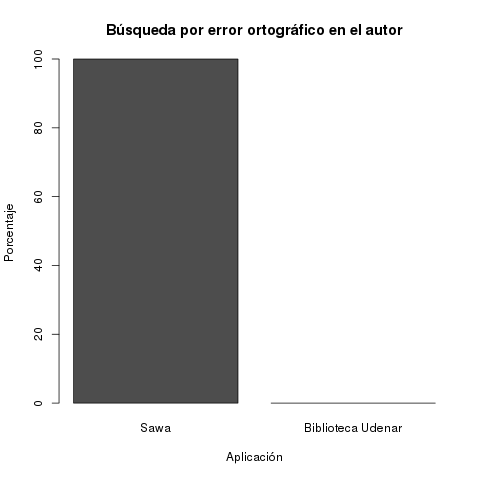
\includegraphics[width=8cm]{pictures/p6.png}
\end{center}
\caption{Búsqueda por error ortográfico en el autor} \label{figura:p6}
\end{figure}

\newpage
 \item [Búsqueda por sinónimos de palabras:] esta búsqueda se la realizó enviando la consulta con algunos de los
 sinónimos de palabras contenidas en el título,  dando como resultado que el sitema realizado
 en esta investigación de un resultado del 80\% y el sistema de biblioteca 0\% como lo muestra la Tabla~\ref{tabla:p7} y Figura~\ref{figura:p7}.
 
 \begin{center}
\begin{table}[!ht]
\caption{Búsqueda por sinónimos de palabras}  \label{tabla:p7}
\scalebox{0.7}{
\begin{tabular}{|c|l |c| c|}
\toprule
\textbf{No} & \textbf{Consulta} & \textbf{SAWA} & \textbf{Biblioteca} \\
\hline
 1 & entendimiento adaptado a una  base bases datos& E & F \\
 \hline
 2 &  intrumento de hallazgo para conocer & E & F \\
 \hline
 3 & elemental hallazgo DE REGLAS & E & F \\
 \hline
 4 & georreferenciación y localización web & E & F\\
 \hline
 5 & geopasto poner tomas de determinación & E & F \\
 \hline
 6 & inspección e informe de archivo o biblioteca & E & F\\
 \hline
 7 & creacion del sistema  para archivo & E & F\\
 \hline
 8 & estudio y creacion de un a red de comunicado & F & F\\
 \hline
 9 & empleo de la asociación cabal& F& F\\
 \hline
 10 & desarrollo de un sistema de inspección para el control escolar & E& F\\
 \hline
\midrule
\bottomrule
\end{tabular}
}
\end{table}
\end{center}
 
   \begin{figure}[!ht]
\begin{center}
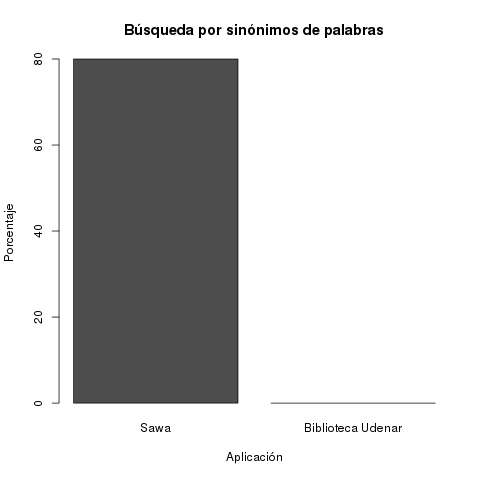
\includegraphics[width=8cm]{pictures/p7.png}
\end{center}
\caption{Búsqueda por sinónimos de palabras} \label{figura:p7}
\end{figure}
 
\end{description}


Se puede mirar el funcionamiento del software y como fueron ejecutadas las pruebas
en el video adjunto  (``Documentacion/Pruebas.mp4'') o en línea\footnote{\url{http://www.youtube.com/watch?v=niE-FcWzp6Q}}.



